%!TEX root = ../dokumentation.tex

%TODO: Einleitungen überarbeiten
\chapter{Konzept}\label{cha:Konzept}
\section{Anforderungen}\label{sec:Anforderungen}
-ermöglichen spielen von spiel mit 2 spielern
-gleichzeitiges chatten möglich
-spielsteine über knöpfe setzen
\section{Übersicht}\label{sec:Übersicht}
Die Anwendung besteht aus zwei verschiedenen Teilen, die beide mittels Docker deployt werden. 
Der eine Teil beinhaltet die Chat-Anwendung und die Spiellogik, der andere beinhaltet eine MongoDB, welche zum Speichern der Benutzer-Login-Informationen verwendet wird.\\
Abbildung \ref{fig:konzept} beinhaltet eine Übersicht über die Komponenten der Anwendung.

\begin{figure}[H]
\centering
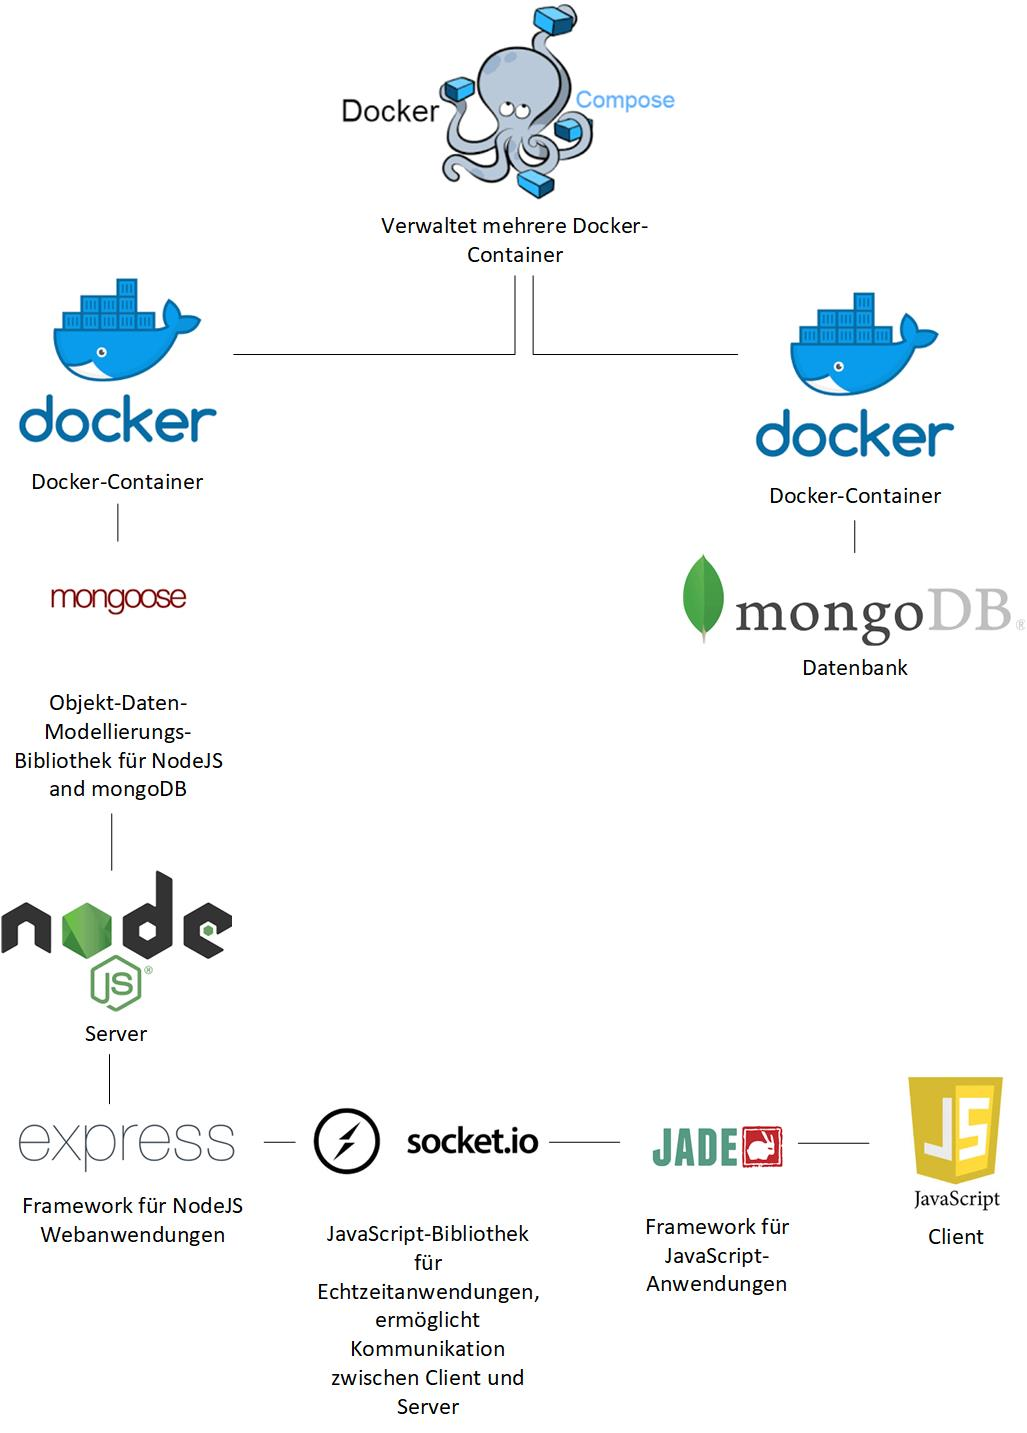
\includegraphics[width=0.75\textwidth]{images/uebersicht.jpg}
\caption{Übersicht der Anwendung}
\label{fig:koncept}
\end{figure}


\section{Login und Registrierung}\label{sec:Login}
Beim Login hat der User die Möglichkeit haben, sich zu registrieren oder sich direkt einzuloggen. 

\section{Spiel}\label{sec:Spiel}

\section{Nachrichtenfilterung}\label{sec:Nachrichtenfilter}
Typischerweise werden bei einer Websocket-Anwendung allen Usern die eintreffenden Nachrichten angezeigt. Um dies zu umgehen und nur den am Spiel beteiligten Spielern relevante Nachrichten anzuzeigen, enthält die Nachricht die Namen der beiden am Spiel beteiligten Parteien. So kann der Client ermitteln, ob er am Spiel beteiligt ist und aufgrund dessen, die Nachrichten anzeigen oder ignorieren. 

\section{Gleichzeitiges Spielen mehrerer Spieler}\label{sec:Multiplegames}
Um es mehr als zwei Spielern zu ermöglichen, gleichzeitig zu spielen, wird eine zweidimensionales Array genutzt. In einer Dimension sind jeweils ein Spielbrett, die zwei Spieler und der Spieler, der aktuell an der Reihe ist, gespeichert. In der anderen Dimension werden die verschiedenen Spiele gespeichert. Sobald ein Spiel beendet wird, werden die zugehörigen Variablen aus dem Array mit dem Wert null belegt. Wenn ein neues Spiel begonnen wird, wird durch das Array iteriert und die erste freie Position verwendet, um dieses Spiel zu speichern. Wenn keine freie Position gefunden werden konnte, das Array erweitert. 

